\subsubsection{UC4 - Selezione \glossario{dizionario dati}}\label{UC4}

\begin{figure}[H]
  \centering
  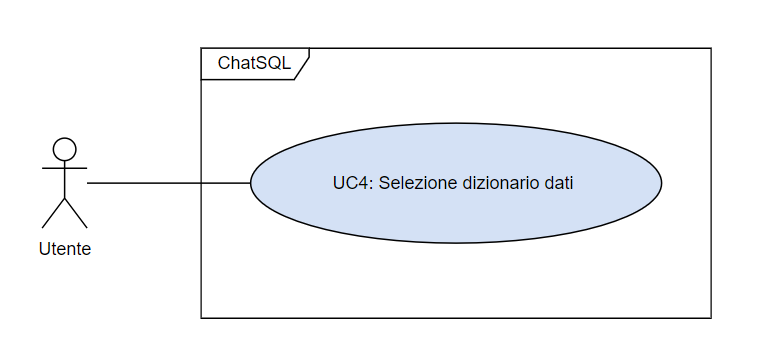
\includegraphics[width=0.90\textwidth]{assets/uc4.png}
  \caption{UC4}
\end{figure}

\paragraph*{Descrizione}
L’Utente desidera selezionare il \glossario{dizionario dati} sul quale basare in seguito l’interrogazione in linguaggio naturale.

\paragraph*{Attori principali}
Utente

\paragraph*{Precondizioni}
\begin{itemize}
  \item L'applicazione è stata avviata con successo;
  \item Nell'applicazione web è stato caricato precedentemente almeno un \glossario{dizionario dati} (\hyperref[UC13]{UC13}).
\end{itemize}

\paragraph*{Postcondizioni}
\begin{itemize}
  \item Un \glossario{dizionario dati} è stato selezionato in modo corretto ed univoco.
\end{itemize}

\paragraph*{Scenario principale}
\begin{enumerate}
  \item L’Utente visualizza la lista dei dizionari disponibili (\hyperref[UC10]{UC10});
  \item L'Utente sceglie un \glossario{dizionario dati} tra quelli presenti.
\end{enumerate}

% Da inserire caso d'errore per l'indisponibilità del dizionario dati